The previous chapter proved what could be proved by looking at every graph of a fixed size. That method is honest and exact, and it stops almost at once. This chapter begins by measuring exactly how fast it stops, because the speed of that collapse is the whole reason a second kind of tool is needed. Then it builds that tool. Where the certifier walks all graphs, the search walks a few of them well, cooling like a physical system toward the densest feasible shape. What it returns is never a proof. It is a concrete graph, hence a lower bound and a conjecture, a stepping stone toward an upper bound that a later proof or certificate must supply. The chapter ends by asking the question any such tool must face: how good is it, and how far from the truth might its answers be.

\section{The wall: how enumeration explodes}

The brute force of \Cref{ch:certify} visits every graph of a given size. The trouble is how many that is. A simple undirected graph on $n$ vertices is a yes-or-no choice on each of the $\binom{n}{2}$ possible edges, so there are $2^{\binom{n}{2}}$ of them. A digraph chooses on each of the $n(n-1)$ ordered pairs, giving $2^{n(n-1)}$, and allowing multiplicities up to a cap $c$ raises the base from two to $c + 1$. These are not numbers that merely grow. They detonate. \Cref{fig:complexity} draws the growth on a logarithmic scale, where each step up the axis multiplies the count tenfold, and the message is the same in every panel: the count passes any reachable budget while $n$ is still in the single digits.

\begin{figure}[ht]
    \centering
    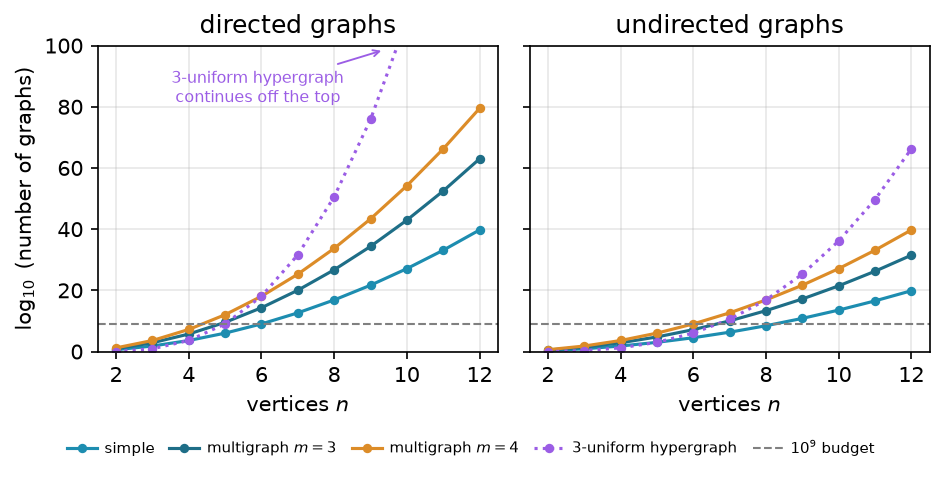
\includegraphics[width=\textwidth]{figures/complexity_growth.png}
    \caption{The number of graphs blind enumeration must visit, on a logarithmic vertical axis, for directed graphs (left) and undirected graphs (right). Each panel shows the simple model, two multigraph connectivity caps, and the three-uniform hypergraph (dotted), with a dashed line at a generous budget of $10^{9}$ candidates, and every curve crosses that budget while $n$ is still in the single digits. Writing $E$ for the number of off-diagonal cells a model may fill, a simple graph offers $2^{E}$ candidates, a multigraph with multiplicity cap $m-1$ (the connectivity ceiling) offers $m^{E}$ (one choice per cell from $\{0,\dots,m-1\}$), and the $3$-uniform hypergraph offers $2^{\binom{n}{3}}$ undirected or $2^{\,n\binom{n-1}{2}}$ directed, since a directed hyperedge is a tail together with two heads. The count depends only on the model and the direction, never on whether one later asks for edge- or vertex-disjoint routes, so a single pair of panels covers all of those variants at once. Direction multiplies the number of cells to fill, by two for graphs (ordered versus unordered pairs) but by three for the $3$-uniform hypergraph, so the directed panel sits far above the undirected one, and the directed cases, exactly the ones \Cref{ch:basecases} left open, are the first to go.}
    \label{fig:complexity}
\end{figure}

Three readings of the figure matter for what follows. Adding vertices is the sharpest cost: each new vertex multiplies the count by an exponential in $n$, so a single extra vertex can move a problem from seconds to centuries. Raising the connectivity budget is the next cost, lifting the base of the exponent rather than its height, which is why the multigraph curves sit above the simple one in every panel. Direction is the third: a digraph has twice as many cells to fill as the undirected graph on the same vertices (and a directed $3$-uniform hyperedge, a tail with two heads, has three times as many), so the directed panel climbs fastest of all, and those are precisely the variants whose answers \Cref{ch:basecases} could not prove. The separation, by contrast, costs nothing here, because edge and vertex disjointness search the same graphs and differ only in what the checker measures, which is why a single pair of panels suffices for all of them. The certifier of \Cref{ch:certify} reaches a few vertices further than blind enumeration, because its cut-counting optimisation is polynomial in the size of the encoding rather than in the number of graphs, but solving that encoding is itself hard and the gain is measured in single vertices, not orders of magnitude. Past that, no exhaustive method reaches the interesting sizes. Something that does not look at every graph is required.

\section{The temperature search}

We want, for fixed $n$ and $m$, a graph with as many edges as possible subject to $\lambda^{\max} \le m - 1$ (or $\kappa^{\max} \le m - 1$ for the vertex variants). The space of graphs on $n$ vertices is enormous and its feasible region has no helpful shape: adding an edge can be harmless until, together with edges added long before, it suddenly creates a forbidden pair. A greedy walk that only ever accepts an improving move stalls at the first such collision, in a graph that is locally maximal but globally far from extremal.

The classical method for this kind of landscape is \emph{simulated annealing} (SA), named after the metallurgical process of cooling a heated material slowly so that its atoms settle into a low-energy crystal rather than a disordered glass. Applied to graphs, annealing escapes local optima by sometimes accepting a worsening move, and by accepting fewer of them as the run proceeds. Each graph $G$ is a state with energy
\[
    E(G) = -|E(G)| + \Lambda \cdot \max\bigl(0,\ \lambda^{\max}(G) - (m - 1)\bigr),
\]
which rewards edges and penalises any excess connectivity. The penalty is a soft constraint rather than a hard one, so the walk may pass briefly through infeasible graphs rather than being walled inside the feasible region, and we return below to why that freedom is worth having. A move toggles one adjacency. The Metropolis rule accepts an improving move always and a worsening move only with probability $e^{-\Delta E / T}$, a chance that shrinks both as the move gets worse and as the temperature drops, and the temperature $T$ falls geometrically, multiplied by a fixed factor just below one at every step. \Cref{alg:anneal} is the whole loop, the one place in this chapter where a body is worth showing, because the loop \emph{is} the method.

\begin{algorithm}[t]
\caption{Temperature search for a dense feasible graph}\label{alg:anneal}
\KwIn{vertices $n$, value $m$, start $T_0$, cooling $\alpha$, penalty $\Lambda$, steps $S$}
\KwOut{the densest feasible graph encountered}
$G \gets$ empty graph on $n$ vertices\;
$T \gets T_0$\;
\For{$S$ steps}{
    propose $G'$ by toggling one adjacency, biasing removals toward low-sensitivity edges\;
    $\Delta \gets E(G') - E(G)$\;
    \If{$\Delta \le 0$ \textbf{or} $\mathrm{rand}() < e^{-\Delta / T}$}{
        $G \gets G'$\;
    }
    \If{$G$ is feasible \textbf{and} denser than the best so far}{
        record $G$ as the best\;
    }
    $T \gets \alpha\, T$\;
}
\Return the best recorded graph\;
\end{algorithm}

This loop is what \code{solve} runs in its discovery mode. With the exhaustive flag off it anneals instead of enumerating, following the Metropolis walk of \Cref{alg:anneal} under geometric cooling, removals biased toward low-sensitivity edges, and returns the densest feasible graph it encountered together with the full temperature trace. What it returns is a witness, hence a lower bound, never a proof.

\codecard{search\_for\_dense\_graph(n, m, variant, separation) $\to$ SearchResult}{DISCOVER}
{the size $n$, the ceiling $m$, the \code{Variant}, the separation, and a step budget}
{a \code{SearchResult}: the densest feasible graph found, with the full step-by-step trace}
{one Metropolis cooling run of \Cref{alg:anneal}. The driver \code{best\_of\_searches} dispatches several independent runs across processor cores and keeps the densest, so a single local optimum never decides the answer.}

It is fair to ask why the walk is allowed above the ceiling at all. Reaching every feasible graph does not require it. Removing an edge can only lower $\lambda^{\max}$ and $\kappa^{\max}$, never raise them, so every subgraph of a feasible graph is again feasible, and the empty graph is feasible trivially. From any feasible target we can therefore delete edges one at a time down to the empty graph without ever crossing the ceiling, and reading that path backward builds the target up the same way. The feasible region is connected through the empty graph by single-edge moves that stay inside it, so a walk that never went infeasible could in principle visit every feasible graph there is.

We let it go infeasible anyway, because reachability and efficiency are different things. A feasible graph can be locally maximal, meaning every edge we might add creates a forbidden pair, and yet still sit far below the densest feasible graph. To improve such a graph the walk has to add an edge and then remove a different one, a swap whose first half is infeasible. A walk confined to feasible graphs could only find that better graph by retreating most of the way back to the empty graph and climbing a different slope, a detour so long that the cooling schedule usually ends first. Allowing a brief excursion above the ceiling lets the walk tunnel straight across instead, trading one load-bearing edge for a better one in two moves rather than dozens. The soft penalty also turns the search into a single smooth landscape with no hard walls for the Metropolis rule to bounce off, and the same machinery then carries over unchanged to variants whose feasible region is not so conveniently connected. Going above the bound is never the goal, then. It is the shortcut the annealer takes on its way back down to it.

\section{Temperature and edge sensitivity}

The phrase ``biasing removals toward low-sensitivity edges'' in \Cref{alg:anneal} is where the temperature acquires its meaning, and it is the heart of the method. For an edge $e$ define its \emph{sensitivity}
\[
    \sigma(e) = \lambda^{\max}(G) - \lambda^{\max}(G - e),
\]
the amount by which deleting $e$ relaxes the binding connectivity. A load-bearing edge sits on a tightest cut and has $\sigma(e) > 0$. Removing it would drop $\lambda^{\max}$ and so loosen the very constraint that limits how many edges the graph may hold. A free edge has $\sigma(e) = 0$: it can be removed without easing the binding pair, which usually means it can be put to better use elsewhere.

\codecard{edge\_sensitivity(G, u, v) $\to \mathbb{N}$}{MEASURE}
{a graph $G$ and one of its edges $e = (u,v)$}
{$\sigma(e) = \lambda^{\max}(G) - \lambda^{\max}(G - e)$}
{delete $e$ and let the checker remeasure, where a positive value marks a load-bearing edge. The whole-graph version \code{sensitivity\_map(G)} reuses one shared baseline measurement. This single number is the dial the cooling turns.}

When the search proposes a removal it draws the edge with probability proportional to $e^{-\sigma(e) / T}$. The dial is now explicit. At high temperature these weights flatten and the walk toggles edges regardless of how load-bearing they are, exploring widely and willing to dismantle essential structure. As the temperature falls the weights concentrate on $\sigma = 0$, so the walk almost never disturbs a load-bearing edge and instead rearranges only the free ones, until the graph crystallises onto an extremal shape. This is exactly the behaviour one wants, and it is the behaviour the formulation asks for: the temperature tracks how strongly removing an edge changes the bound. \Cref{fig:trace} shows one such run settling onto a certified optimum. \Cref{app:traces} collects five further traces, covering both matrix models in both directions and one run under the vertex separation, and the behaviour is the same in each.

\begin{figure}[ht]
    \centering
    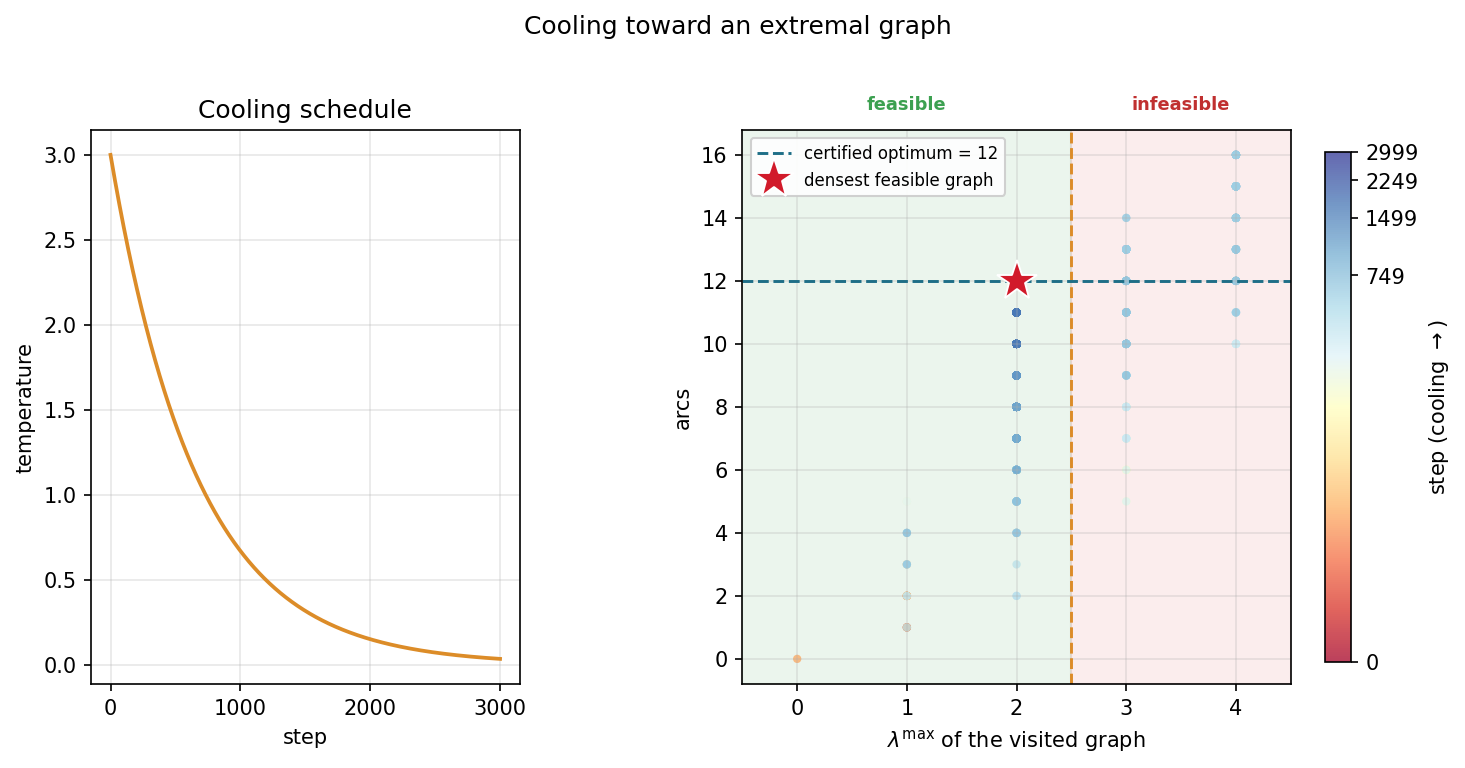
\includegraphics[width=0.78\textwidth]{figures/temperature_trace.png}
    \caption{A single cooling run on the directed multigraph problem at $n = 4$, $m = 3$. \emph{Left:} the temperature schedule, cooling geometrically from its starting value. \emph{Right:} every visited graph plotted by its binding connectivity $\lambda^{\max}$ (horizontal) against its arc count (vertical), coloured by the step at which it was visited. Annealing uses a soft penalty rather than a hard wall, so while hot (dark points) the walk strays into the infeasible region $\lambda^{\max} > m - 1 = 2$, picking up extra arcs it is not allowed to keep. As the temperature falls (bright points) the penalty drives the walk back across the feasibility boundary and onto the densest graph that stays feasible, the certified optimum of $12$ arcs at $\lambda^{\max} = 2$ (star).}
    \label{fig:trace}
\end{figure}

The same sensitivities also explain a finished graph. Colouring a graph's arcs by $\sigma$ shows at a glance which arcs are structural and which are slack. \Cref{fig:sensitivity} illustrates all four sensitivity levels on one directed multigraph: the darkest arcs carry the most flow and lower $\lambda^{\max}$ the most when removed, the cool arc contributes nothing. The picture is not decoration: it is the certificate of tightness made visible, and it tells the search exactly which arcs to leave alone as the temperature falls.

\begin{figure}[ht]
    \centering
    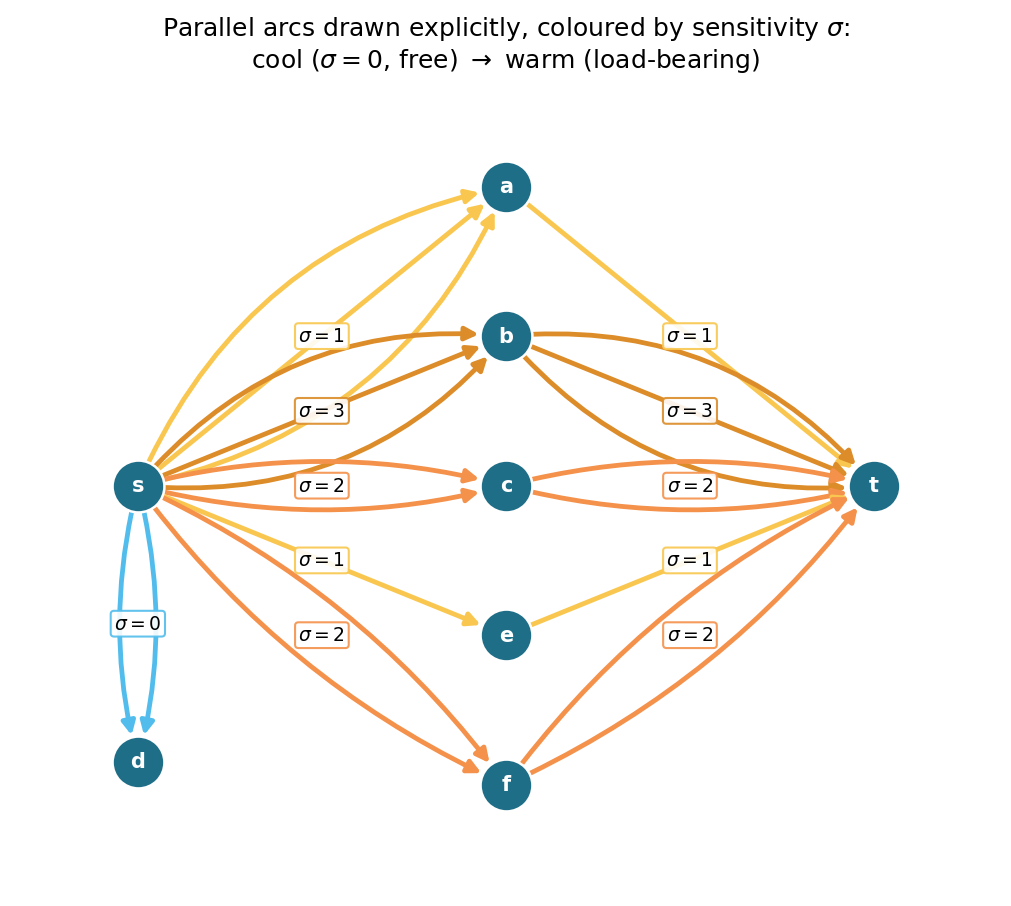
\includegraphics[width=0.78\textwidth]{figures/sensitivity_mixed.png}
    \caption{A directed multigraph on eight vertices with $\lambda^{\max} = 9$, every parallel arc drawn explicitly and coloured by its sensitivity $\sigma$, so multiplicity is read by counting arcs rather than from a label. The point is the contrast between $s \to a$ and $s \to b$: both carry three parallel arcs, yet $s \to a$ is cool ($\sigma = 1$) because the single arc $a \to t$ downstream throttles that route to one unit, while $s \to b$ is hot ($\sigma = 3$) because all three of its copies carry flow. The arcs $s \to d$ are coolest of all ($\sigma = 0$): $d$ is a dead end, so deleting them changes nothing. Removing a hot adjacency drops $\lambda^{\max}$ by its $\sigma$ while removing a cool one does not, which is exactly what tells the search which arcs to leave alone as the temperature falls.}
    \label{fig:sensitivity}
\end{figure}

A single cooling schedule can still settle into a local optimum, so in discovery mode \code{solve} runs several independent schedules from different starting seeds and keeps the densest result across all of them. Because the restarts share no state and none depends on the outcome of another, they run in parallel. The program dispatches them across the available processor cores, so the wall-clock cost of $k$ restarts is a small multiple of a single run rather than $k$ times it, bounded below by the slowest restart and by the cost of starting the worker processes. A handful of parallel restarts is enough to reach the known optima at the sizes we examine. This is a reliability measure, not a change of method, and the parallelism is invisible to every number the thesis reports: the same best graph would be found by running the schedules sequentially, just more slowly.

\section{Keeping the checker cheap inside the search}

The energy of \Cref{alg:anneal} reads the binding connectivity $\lambda^{\max}(G)$, and a literal reading of the loop would call the checker afresh on the whole graph at every step. That checker is the most expensive routine in the program, one maximum flow per ordered pair, and the walk runs for thousands of steps with several restarts, so such a search would spend nearly all of its time remeasuring graphs that barely changed from the step before. Two elementary facts remove almost all of that work without altering a single number the search reports.

\begin{proposition}[Monotonicity of the binding connectivity]\label{prop:monotone}
Let $G$ be a graph or directed multigraph, and let $G'$ be obtained from $G$ by changing one adjacency by a single unit of multiplicity. Then
% The prose below cites these as "part (1)" and "part (2)", so this list
% carries explicit numbers in place of the decorative global list icon.
\begin{enumerate}[label=(\arabic*)]
    \item \textup{(monotonicity)} removing the unit cannot raise $\lambda^{\max}$, and adding it cannot lower $\lambda^{\max}$, and
    \item \textup{(unit step)} adding the unit raises $\lambda^{\max}$ by at most one.
\end{enumerate}
Both statements hold verbatim for the vertex measure $\kappa^{\max}$.
\end{proposition}

\begin{proof}
Fix an ordered pair $(s,t)$. By the max-flow / min-cut theorem $\lambda_G(s,t)$ is the smallest capacity of any cut separating $s$ from $t$, where the capacity of a cut is the total multiplicity of the arcs that cross it from the source side to the sink side.

For part (1), reducing one adjacency by a unit lowers the capacity of every cut that the changed arc crosses and leaves all other cut capacities untouched, so no cut capacity rises. The smallest cut capacity therefore cannot rise either, which gives $\lambda_{G'}(s,t) \le \lambda_G(s,t)$. Taking the maximum over all pairs yields $\lambda^{\max}(G') \le \lambda^{\max}(G)$. Adding a unit is the same statement read backwards.

For part (2), write $G''$ for $G$ with one unit added to a single adjacency. That extra unit of capacity crosses any fixed cut at most once, so every cut has capacity at most one greater in $G''$ than in $G$. The smallest cut capacity thus grows by at most one, giving $\lambda_{G''}(s,t) \le \lambda_G(s,t) + 1$, and together with part (1) we have $\lambda_G(s,t) \le \lambda_{G''}(s,t) \le \lambda_G(s,t) + 1$. The maximum over pairs gives $\lambda^{\max}(G'') \le \lambda^{\max}(G) + 1$.

For $\kappa^{\max}$ the argument is identical on the vertex-split network of \Cref{fig:vertex-split}, where changing an adjacency changes the capacity of its single arc $u^{\mathrm{out}} \to v^{\mathrm{in}}$ in the same way. Parallel copies leave that capacity at one and so change $\kappa^{\max}$ not at all, which only strengthens both parts.
\end{proof}

These two facts settle almost every step without a flow. The energy depends on $\lambda^{\max}$ only through the excess $\max(0,\ \lambda^{\max} - (m-1))$, which is zero exactly when the graph is feasible. So a removal applied to a feasible graph leaves it feasible by part (1), with excess still zero, and needs no measurement at all. An addition made while the graph sits strictly below the bound, at $\lambda^{\max} \le m - 2$, stays feasible by part (2), which caps the rise from a single added unit at one, so the graph can move at most to $\lambda^{\max} = m - 1$, still inside the feasible region, again with excess zero and no measurement. Only an addition made right at the boundary $\lambda^{\max} = m - 1$ can tip the graph over, and only there does the search run a single flow, capped so that it stops the instant it finds one route too many. The exact connectivity value is recomputed only on the rare step whose proposal is genuinely infeasible, where the penalty term needs it. The three cases of \Cref{prop:monotone} read directly off the code:

\begin{lstlisting}[caption={The three cases behind \Cref{prop:monotone}, in the order the proof gives them: removal from a feasible graph (part 1), addition below the bound (part 2), and only otherwise a single capped flow.}, label={lst:capped-energy}]
if (is_add and lam_ub <= m - 2) or (not is_add and feasible_current):
    excess = 0                # part (2) or part (1): provably feasible
elif not exceeds_bound(proposal, m - 1, separation=separation):
    excess = 0                # at the boundary, but the flow clears it
else:
    excess = measure_full(proposal) - (m - 1)   # infeasible: exact penalty
\end{lstlisting}

To know which case applies, the search carries a running upper bound on $\lambda^{\max}$, raised by one whenever it accepts an addition (part (2)) and left untouched when it accepts a removal (part (1)), and resynchronised to the exact value at the cadence where it already pays for flows to refresh the sensitivity map. The bound can only ever sit at or above the truth, so any step it clears is certainly feasible.

The key point is that the energy returned on every step is, by \Cref{prop:monotone}, exactly the value the naive implementation would have computed. Every accept-or-reject decision, every random draw, and the graph the walk finally returns are therefore unchanged, and the speed-up is invisible to every number the thesis reports. This is verified rather than asserted. A regression test runs both implementations, the fast one and a reference that measures exactly at every step, across all four graph variants and both separations, and checks that the two agree step for step in energy, in every accept-or-reject decision, and in the final graph, and that the returned graph is feasible under the exact checker. Nothing about the optimisation hides inside the bound: the witness the search reports is always certified by an exact measurement, exactly as in the slower search.

It is worth noting where this method earns its keep. For undirected graphs one could resynchronise the exact value cheaply from the Gomory--Hu tree of \Cref{ch:certify}, which encodes every pairwise edge-connectivity in $n - 1$ flows. The directed and vertex variants admit no such tree, so there the monotone bound and the capped predicate are the only inexpensive handle on feasibility, and they are what let one annealer serve every variant at speed.

\section{Rediscovering the known extremisers}

A search method is only worth trusting if it recovers what is already known before it is pointed at what is not. Run from the empty graph on the cases whose answers \Cref{ch:basecases} and \Cref{ch:certify} settled, and told only to pack in edges without breaching the connectivity ceiling, the cooled search arrives unprompted at the named constructions. \Cref{tab:rediscovery} reports the densest graph it found against the value the theory predicts, and in every case the two agree.

\begin{table}[t]
    \centering
    \begin{tabular}{lrrrrrr}
\toprule
Variant & $n$ & $m$ & Limit (s) & Elapsed (s) & Search & Optimum \\
\midrule
simple undirected & 6 & 2 & 2 & 2.006 & 5 & 5 \\
multi undirected & 6 & 3 & 2 & 2.004 & 10 & 10 \\
simple directed & 4 & 2 & 2 & 2.000 & 6 & 6 \\
simple directed & 6 & 2 & 2 & 2.020 & 10 & 10 \\
simple directed & 7 & 2 & 2 & 2.022 & 12 & 12 \\
multi directed & 4 & 3 & 2 & 2.000 & 12 & 12 \\
multi directed & 5 & 3 & 2 & 2.011 & 16 & 16 \\
\bottomrule
\end{tabular}

    \caption{Validation by rediscovery. For each variant the temperature search, run from scratch with a handful of restarts, recovers exactly the extremal value proved or certified in the earlier chapters. The ``Search'' column is an honest lower bound found by annealing, and the ``Theory'' column is the proved or certified value.}
    \label{tab:rediscovery}
\end{table}

What the table hides is that the graphs themselves are the named constructions, not merely graphs of the right size. The simple undirected run at $m = 2$ settles on a spanning tree, the only shape with $n - 1$ edges and no cycle. The undirected multigraph run settles on a star with every edge at multiplicity $m - 1$, an instance of the multi-tree extremiser behind \Cref{thm:multigraph-edge}. The directed multigraph runs settle on the double star of \Cref{ch:certify}, both directions of every spoke at full multiplicity. The simple directed runs find the bidirected star at $n = 4$ and, at $n = 7$, land on twelve arcs, the value at which the hub and the one-directional wall tie, exactly the crossover \Cref{thm:dir-arc-m2-exact} predicts. The cooled search does not know these names. It rediscovers the structures because, under the connectivity ceiling, there is nowhere denser to go.

Some extremisers are past the size at which a quick search lands reliably, but the exact checker of \Cref{ch:certify} settles them immediately by measuring their connectivity. The one-directional bipartite digraph on eight vertices has $16$ arcs at $\lambda^{\max} = 1$, and $16$ already exceeds the linear hub value $2(n-1) = 14$: the smallest size at which the quadratic phenomenon strictly wins, made concrete. It is also a measured illustration of the search's limit: repeated cooling runs at $n = 8$, $m = 2$ stall at the hub value of $14$, because dismantling a finished hub and rebuilding a one-directional wall is far more than the single-arc moves of the walk can tunnel through. The known answer there comes from the construction and the checker, not from the search, which is exactly the division of labour this chapter argues for. The augmented bipartite digraph on ten vertices at $m = 3$ has $30$ arcs at $\lambda^{\max} = 2$, the thirty-arc counterexample of \Cref{rem:counterexample-m3}, confirmed pair by pair against the naive bound of $27$ it refutes. The directed double star on seven vertices at $m = 4$ has $36$ arcs at $\lambda^{\max} = 3$, matching $2(n-1)(m-1)$. None of these is a proof of optimality. Each is an exactly measured feasible graph, a lower bound the checker stamps as genuine.

\subsection{Simulated annealing versus tabu search}

The annealer is not the only way to walk this landscape. A natural alternative, suggested by Jan Goedgebeur, is \emph{tabu search} (\Cref{tab:functions} names the implementation), which keeps the energy and the neighbourhood of \Cref{alg:anneal} but replaces the cooling schedule with a deterministic best-improving step. At each step it evaluates every single-edge move from the current graph and takes the one that lowers the energy most, then forbids the pair it just changed for a fixed number of steps, the \emph{tabu tenure}, so the walk cannot immediately undo its last move and stall in a two-step cycle. When no improving move is left and the search stalls, it perturbs the incumbent with a few random moves and carries on. There is no temperature and no accept-worse coin: apart from the perturbation kicks the walk is deterministic. Where annealing explores by occasionally stepping uphill and trusts the cooling to settle it, tabu climbs greedily and trusts the tabu list to keep it from retracing its path.

The two engines rediscover the same values, but at very different speeds, and on the harder directed cases the difference is decisive. \Cref{tab:sa-vs-tabu} runs them head to head at an equal budget of six seconds each, both restarted within that budget. On the simple undirected problem both reach the optimum at once. On the two directed problems past the certified range tabu reaches the optimum within the budget while the annealer plateaus below it, assembling the eighteen-arc simple-directed extremiser and the full twenty-four-arc double star at $n = 7$ where the annealer stalls at sixteen and twenty. The cause is the one already met at the $n = 8$, $m = 2$ hub stall above. The annealer cools onto whatever dense shape it first reaches and then cannot dismantle it within the budget, whereas tabu's best-improving step follows the steepest density gradient and the tabu list stops it sliding back, so it assembles the structured extremiser the cooled walk struggles to find.

\begin{table}[ht]
    \centering
    \begin{tabular}{lllrrrcc}
        \toprule
         & & & & \multicolumn{2}{c}{best in $6$\,s} & \multicolumn{2}{c}{time to optimum} \\
        \cmidrule(lr){5-6}\cmidrule(lr){7-8}
        Variant & $n$ & $m$ & optimum & SA & tabu & SA & tabu \\
        \midrule
        simple undirected   & 7 & 3 & $9$  & $9$  & $9$  & $1.3$\,s & $0.1$\,s \\
        simple directed     & 7 & 3 & $18$ & $16$ & $18$ & ---      & $2.6$\,s \\
        directed multigraph & 7 & 3 & $24$ & $20$ & $24$ & ---      & $2.5$\,s \\
        \bottomrule
    \end{tabular}
    \caption{Simulated annealing (SA) against tabu search at an equal six-second budget per method, all at $m = 3$, the annealer restarted from fresh seeds and tabu restarted on stalls. Only the simple undirected value is a proved optimum (Mader). The two directed values are the best known rather than proved, found by search and construction past the certified range that stops below $n = 7$ for those variants (\Cref{sec:trichotomy}), so here the ``optimum'' column is the target each engine is trying to reach. Both reach the simple undirected optimum. On the two directed problems tabu reaches the best known value while the annealer plateaus below it. The last two columns give the wall-clock time each method first reached that value on the reference machine, with a dash where it did not reach it in the budget.}
    \label{tab:sa-vs-tabu}
\end{table}

\Cref{fig:sa-vs-tabu} shows the divergence directly, plotting the densest feasible graph each engine has found against wall-clock time on the two directed multigraph cases. Tabu climbs in a few decisive steps and holds at the optimum, while a single annealing schedule rises quickly and then flattens a few arcs below it. The annealer's independent restarts recover the optimum on the smaller case, as \Cref{tab:rediscovery} records, so a single plateau is not the whole story there. But at $n = 7$ the plateau persists within the budget, and one tabu schedule already reaches what the restarted annealer does not.

\begin{figure}[ht]
    \centering
    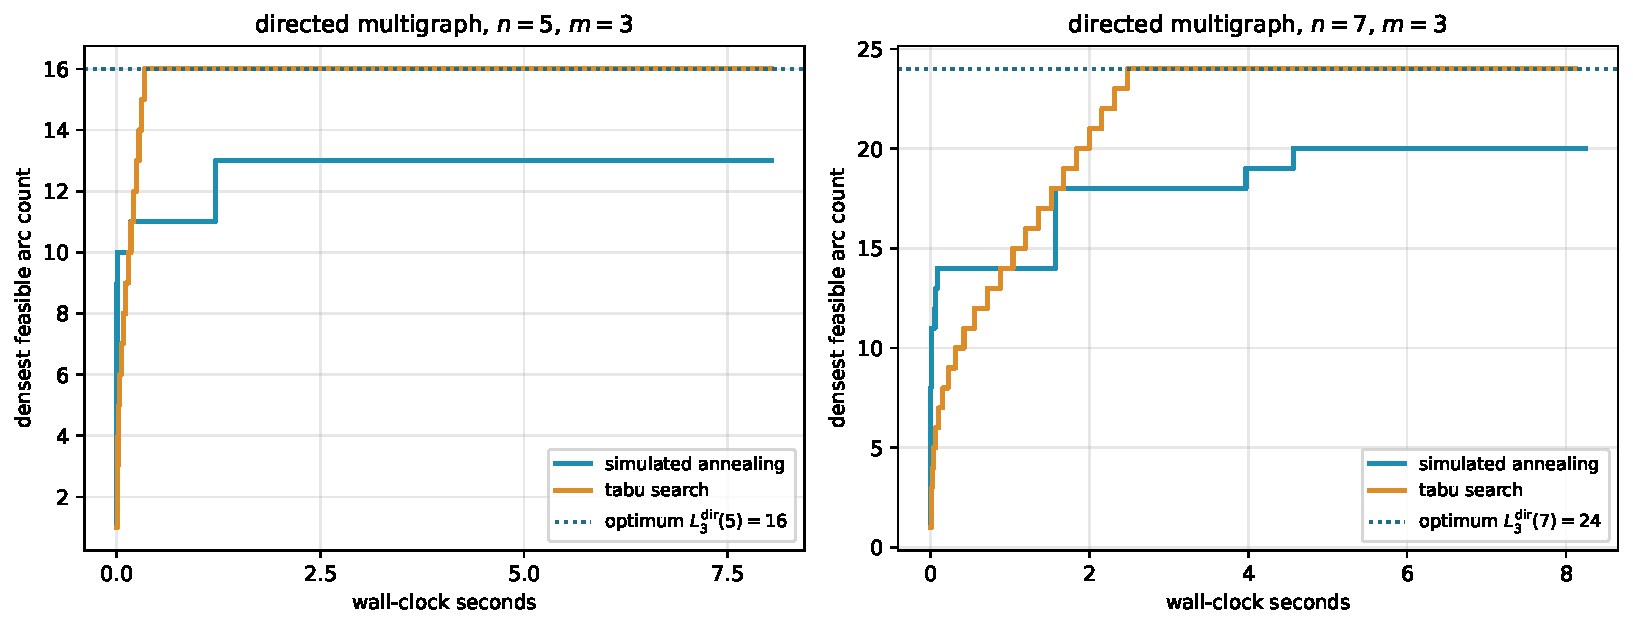
\includegraphics[width=\textwidth]{figures/sa_vs_tabu_convergence.pdf}
    \caption{Densest feasible graph found against wall-clock time, for one simulated-annealing schedule and one tabu schedule on the directed multigraph at $n = 5$ and $n = 7$, $m = 3$. Tabu climbs in a few best-improving steps to the optimum (dotted) and holds, while a single annealing schedule rises quickly and then flattens below it. The time axis is wall-clock on the reference machine, so unlike the seed-reproducible figures elsewhere this one is a representative timed run.}
    \label{fig:sa-vs-tabu}
\end{figure}

This advantage comes at a cost the equal-time comparison already absorbs but is worth naming: each tabu step scans the whole neighbourhood, so it is far more expensive than the annealer's single random proposal, and tabu takes many fewer but better-aimed steps in the same wall-clock. Tabu search is therefore the program's default for solving the problems, reaching every value this thesis reports, the rediscovery of \Cref{tab:rediscovery} and the conjectural lower bounds alike, and reaching the harder directed optima past the certified range where the annealer plateaus. Simulated annealing is kept for the self-check and verification, where the small values fall at once, the lighter per-step cost is all that is needed, and its independent restarts parallelise trivially across cores.

\section{The trichotomy: proved, certified, conjectured}
\label{sec:trichotomy}

It is worth stopping to lay out, for every variant, the three kinds of knowledge the computation can hold about it, because the whole value of the pipeline is that they are kept apart and never quietly merged. About any given value the program can do one of three things. It can \emph{prove} the value, closing a fixed size from above by exhausting every graph of that size, an upper bound with the standing of a hand proof. It can \emph{certify} it, the same kind of upper bound but obtained by the cut-counting optimisation rather than blind exhaustion, reaching a vertex or two further. Or, where proof and certificate both run out, it can only \emph{conjecture} the value, exhibiting a concrete dense graph that pins down a lower bound and leaving the matching upper bound to a later argument.

Proof and certificate bound the answer from above. The search bounds it only from below. Where a closed \emph{formula} exists it can tie the two together, threading through the certified small cases and the conjectured large ones as a single curve. This is the discipline the whole thesis runs on, and it is worth stating as one: the search proposes a lower bound, a certificate or a hand proof disposes the upper bound, and only when both meet is a value called settled.

We begin with the single variant where all three kinds of knowledge are non-trivial and visibly distinct, the directed simple arc problem at a fixed $m \ge 3$, and then sweep the whole family. For that variant the knowledge splits cleanly by the size of the graph.

For small $n$ the answer is not conjectured at all. The pruned exhaustion inside \code{solve} walks every simple digraph on $n$ vertices and returns the exact maximum, complete and certain, an upper bound with the standing of a hand proof. At $m = 3$ it certifies $6, 9, 12$ for $n = 3, 4, 5$, and there the exhaustion stops within a reasonable budget, the pruned walk no longer closing $n = 6$ in tractable time. That is the certified region, finite and closed.

Beyond it the ceiling is gone and only lower bounds remain, each witnessed by a concrete feasible graph. The search finds the extremal $15$ arcs at $n = 6$ on its own. Past that size it falls behind: across six restarts it reaches $17, 17, 20, 23$ for $n = 7, \dots, 10$, while the named constructions of \Cref{ch:basecases}, measured exactly by the checker, supply $18, 21, 25, 30$, the last being the thirty-arc graph of \Cref{rem:counterexample-m3}. The reported lower bound at each size is the better of the two, exactly as the rediscovery section combined search and checker by hand. These are conjectures with an honest floor and no matching ceiling. That is the searched region, unbounded and forever one-sided.

The two regions are tied together by a single closed form. The conjectured value
\[
    \ell_m^{\mathrm{dir}}(n) = \max\!\left(m(n-1),\ \floorfrac{(n+m-2)^2}{4}\right)
    \qquad (n \ge m)
\]
of \Cref{conj:dir-arc} is not a fresh guess bolted on past the certified range. It is one formula that already passes through every certified value at small $n$ and then continues, without a seam, through every searched value at large $n$. The directed-arc panels of \Cref{fig:variant-bounds-m3} show this directly: the certified squares, proved exactly at the small sizes the certifier reaches, sit on the one red conjecture curve there, and the open lower-bound circles, the best feasible graph the search finds at each larger size, sit on that same curve past that point, matching it as far out as the search goes without ever crossing above it. The formula is the through-line that makes the small certified cases and the large conjectured ones a single statement rather than two.

Two features of those directed-arc panels are worth naming. The crossover from the linear hub term to the quadratic bipartite term happens at $n = 9$, where the second argument of the maximum first wins, and that is past the last certified size. The shape of the answer therefore changes in exactly the region where only the search can see it, which is precisely why a discovery tool was needed and a certifier alone would not do. And at $n = 10$ the formula reads $30$, the count of the very counterexample that overturned the natural initial conjecture, so the closed form is not a smooth fit to easy data but one that survives the case that broke the previous guess.

Asking the same three questions of every variant, the answers sort into three regimes, and \Cref{fig:variant-bounds-m3} shows all twelve at once, one panel per variant, in exactly this proved, conjectured, and guessed language.

In the first regime the closed form is already a theorem for every $n$, proved by hand in \Cref{ch:basecases} or cited, and the computation only confirms it. The undirected edge families live here for every $m$, together with the directed problems at $m = 2$ and, up to a threshold in $m$ that differs by model, the undirected vertex families as well: through $m \le 4$ for simple graphs and multigraphs (\Cref{thm:leonard}) and through $m \le 3$ for hypergraphs (\Cref{thm:hyper-vertex-m2,thm:hyper-vertex-m3}). Past those thresholds the same rows drop into the third regime below, which is why the leaf colours of \Cref{fig:variant-tree-status} are stated at general $m$ and \Cref{tab:summary} carries the exact ranges. For these the certified small cases and the rediscovered constructions of \Cref{tab:rediscovery} are validation, not new knowledge: the formula was never in doubt, and the program's role is to check that the pipeline reproduces it. That the two multigraph vertex rows measure exactly as their underlying simple graphs is a matter of the counting convention of \Cref{sec:parallel-convention} rather than a theorem, so those rows need no computation of their own at all. The directed vertex rows do need their own computation. Whitney's inequality $\kappa^{\max} \le \lambda^{\max}$ means every graph feasible for the arc problem is automatically feasible for the vertex problem too, since a small $\lambda^{\max}$ forces an even smaller $\kappa^{\max}$. So the arc problem's own dense construction doubles as a valid witness, hence a lower bound, for the vertex problem. But it supplies no upper bound: a bound proved only for the smaller arc-feasible family says nothing about the larger vertex-feasible family, which may contain denser graphs the arc argument never had to rule out. So they get their own: every exact point on those panels comes from the search and the exhaustion run under the vertex test.

In the second regime the three columns genuinely differ and the computation is load-bearing. This is the regime of the worked example above. The directed simple arc and vertex problems at $m \ge 3$ are certified only at the small $n$ the exhaustion reaches and conjectured by the search beyond, with the formula of \Cref{conj:dir-arc} the through-line.

The directed multigraph arc problem used to sit here and no longer does. It has moved up into the first regime, since \Cref{thm:dir-multi-full} proves $L_m^{\mathrm{dir}}(n) = (m-1)\max(2(n-1), \floor{n^2/4})$ for every $n$ and every $m$, with no parity split and no auxiliary conjecture. Its panel is worth watching all the same, because it is the one place in the grid where the computation and the proof were developed against each other rather than in sequence: in its cut-counting mode \code{solve} proves the $m$-free number $M^{*}(n) = 2(n-1)$ outright for $n \le 6$, and the scaling identity $L_m^{\mathrm{dir}}(n) = (m-1)\,M^{*}(n)$ of \Cref{ch:certify} carries that one certified number to every $m$ at once. Those certificates were the evidence that the closed form was right long before the proof of it existed, and they now serve as an independent check on a theorem rather than as the reason to believe a conjecture.

In every row of this regime the formula agrees with proof where proof reaches and with the search where it does not, exactly the linkage the worked example displayed.

In the third regime there is no formula at all, and the honesty is in drawing the guess as a guess. The undirected vertex problem at $m \ge 6$ has been open since 1974 with its extremal structure genuinely unknown. The undirected hypergraph vertex problem joins it, but only from $m \ge 4$: at $m \le 3$ its value is settled for every uniformity and every $n$ (\Cref{thm:hyper-vertex-m2,thm:hyper-vertex-m3}), which is why that panel of \Cref{fig:variant-bounds-m3} carries a proved blue curve while its counterpart in \Cref{fig:variant-bounds-m6} carries a yellow guess. The two \emph{directed} hypergraph variants are in the third regime at every $m$, and they need a one-tail, many-head reading of a Berge edge that this thesis defines itself only so that \code{solve} can measure it at all. Here the program still computes exact values at the few sizes that finish, and its search still exhibits feasible graphs at a handful more, but no closed form is in sight. What is known there is asymptotic rather than exact: \Cref{thm:dir-hyper-constant} pins the leading term at $(m-1)n^2/(4(r-1))$ for both separations, which is a statement about where these curves are heading and not one a panel at $n \le 10$ can display. The panels of \Cref{fig:variant-bounds-m3} carry, instead of a red conjecture curve, a yellow line that simply interpolates the machine points in straight segments, trusted no further than the eye. We draw it \emph{through} the points rather than fitting a smooth curve above them: the points are honest lower bounds, the truth lies on or above them, and a line riding above the points would claim more than the search ever found.

Two cautions govern how to read the dotted curves. At small $n$ the complete graph or hypergraph is itself feasible, its binding connectivity being only $n - 1$, so the earliest points merely trace the trivial maximum and reveal nothing of the open behaviour: the undirected-vertex points run up $\binom{n}{2}$ until $n$ passes $m$, and only then bend toward the linear growth the proved edge value predicts.

Past that bend the dotted line is as strong as the best lower bound behind it, which at each size is the better of the quick search and a named construction the checker verifies. The search alone stalls, exactly as it stalled on the quadratic wall in the rediscovery above: where it cannot build a denser construction its own reports climb only linearly. The clearest case is the directed hypergraph, whose bipartite family is quadratic, reaching ${\sim}\,(m-1)n^2/\bigl(4(r-1)\bigr)$ hyperarcs by \Cref{prop:dir-hyper-first}: there the walk slips below that construction at larger $n$, so it is the construction that carries the circles, with the search free to beat it wherever it can. We therefore read the dotted trends as honest lower bounds and not as fitted laws, and the one closed form we record on those panels, the quadratic for the directed hypergraph, comes from the construction and not from the shape of the dots. That it is also the right leading term is a theorem (\Cref{thm:dir-hyper-constant}), which is a fact about the construction rather than about the dots.

So to the question of whether one formula links what is proved to what is conjectured, the answer is three-valued and depends on the variant, and the grid of \Cref{fig:variant-bounds-m3} shows all three at a glance. Where the problem is already solved the curve is blue, a theorem the computation merely agrees with. Where the problem is open but tractable the curve is red, a conjecture the certified squares confirm exactly at the small sizes the certifier reaches and the searched circles confirm, without proving, at every larger size the search reaches, and that is the case the program was built for. Where the problem is genuinely hard the curve is yellow, a guess interpolated through the search points and an open question of what, if anything, the dots truly trace.

One feature stands out in the bottom row: the directed hypergraph panels, both arc and vertex, climb steeply at $m = 3$, the yellow guess curving upward rather than running straight. This is genuine and not search instability: the directed Berge edge packs a tail and $r-1$ heads into a single object, and the bipartite construction of \Cref{prop:dir-hyper-first} already reaches roughly $(m-1)n^2/(4(r-1))$ hyperarcs, so the value grows with $n^2$. The same quadratic shape sits one column over, in the directed arc and vertex panels, whose conjectured red curves carry the $\floorfrac{(n+m-2)^2}{4}$ term and rise just as fast. Super-linear growth is the signature of \emph{direction} across the grid, not of the hypergraph alone: every directed column bends upward while the two undirected columns stay linear. \Cref{fig:variant-bounds-m6} redraws the same grid at $m = 6$: the proved curves climb linearly with $m$ exactly as their formulas predict, while the open variants' search points and their yellow interpolation climb higher without a proved curve to meet, so raising the threshold does not change which regime a variant lives in, only how far the red and yellow curves have travelled.

\begin{figure}[htbp]
    \centering
    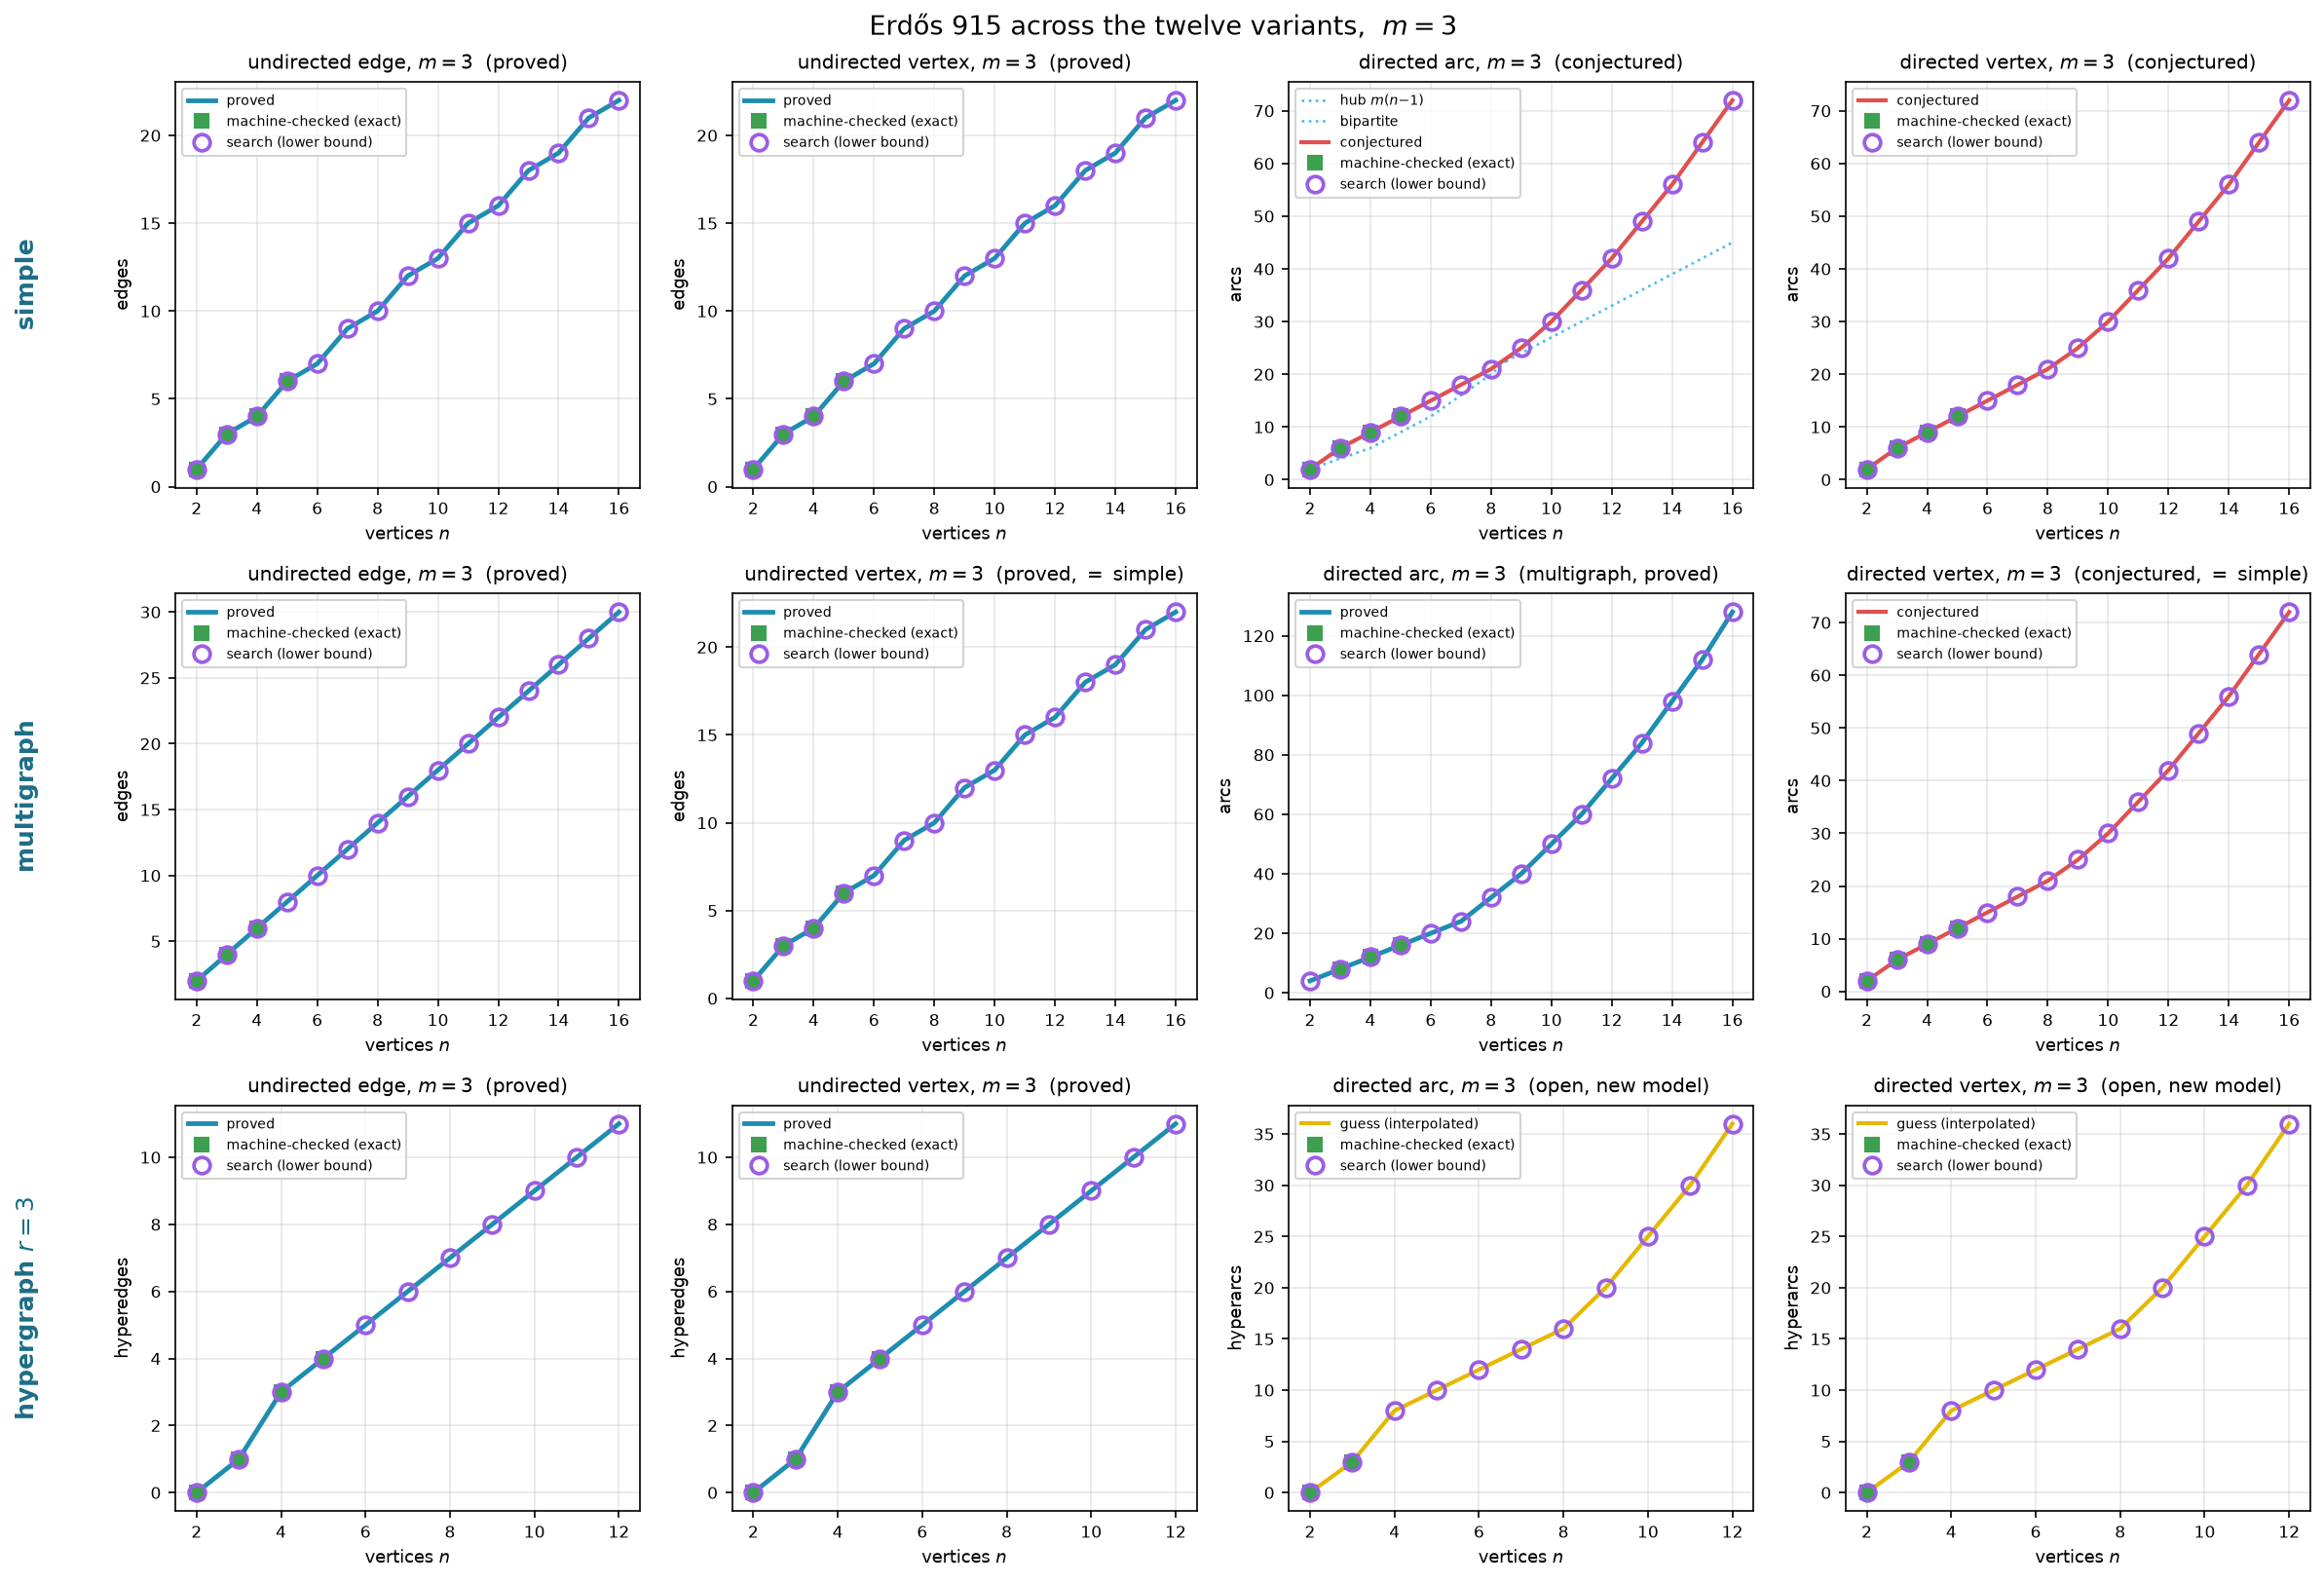
\includegraphics[width=\textwidth]{figures/variant_bounds_m3.png}
    \caption{All twelve variants at $m = 3$, edges against $n$, laid out by model (rows: simple, multigraph, $3$-uniform hypergraph) and by separation and direction (columns: undirected edge, undirected vertex, directed arc, directed vertex). A \emph{blue} curve is a value proved for all $n$, a \emph{red} curve a conjectured formula, and a \emph{yellow} curve a bare interpolation of the machine points where no formula is known, the three told apart by colour rather than by dash pattern. Filled squares are the sizes \code{solve} proved or certified exactly. Open circles are lower bounds at larger $n$, the better at each size of the search's densest find and a named construction measured by the checker, reported as a running maximum so a feasible graph at one size is never lost at the next. On the open variants the yellow curve is the piecewise-linear interpolation \emph{through} those circles, never above them, and the axes are scaled to the data rather than to a loose certain interval. The directed hypergraph panels in the bottom row rise steeply because their value is quadratic in $n$, not linear.}
    \label{fig:variant-bounds-m3}
\end{figure}

\begin{figure}[htbp]
    \centering
    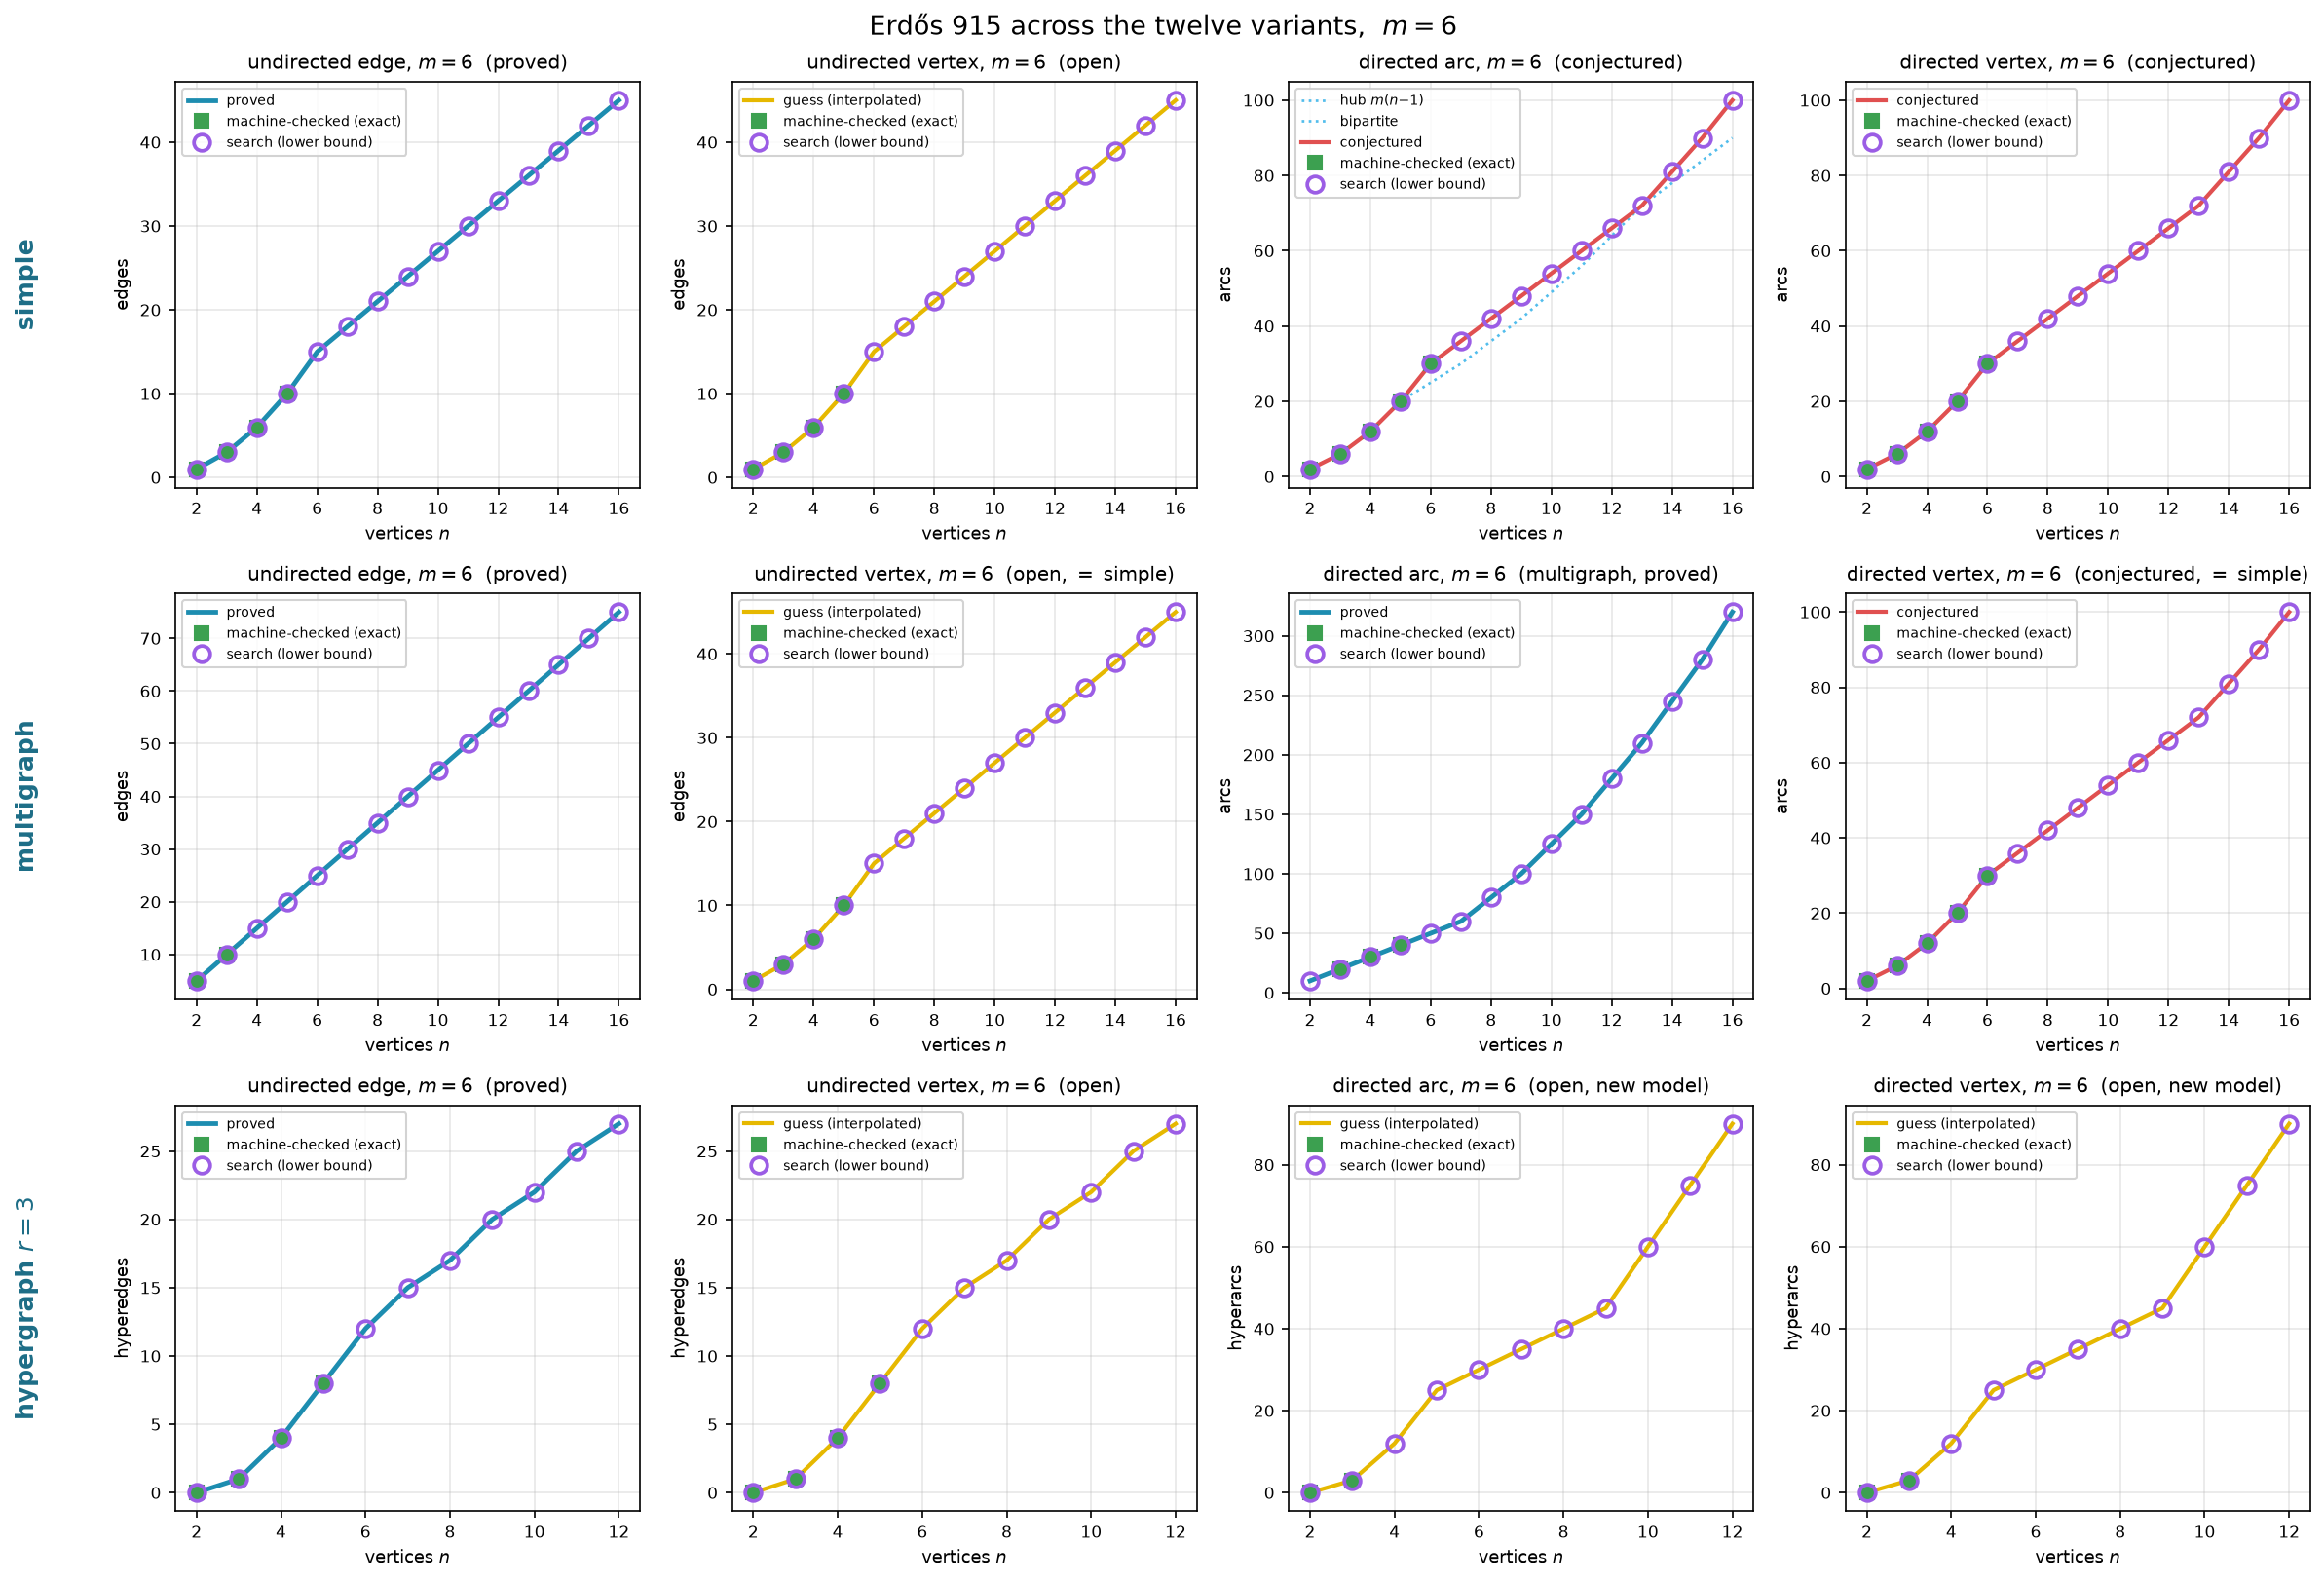
\includegraphics[width=\textwidth]{figures/variant_bounds_m6.png}
    \caption{The same twelve variants at $m = 6$. The undirected edge and multigraph edge cases remain proved (Mader's theorem holds for all $m$), while the undirected vertex separation is the famous open problem at $m \geq 5$ and the directed cases carry the same conjectured formula scaled to $m = 6$. On the open vertex panels the circles never sit below the proved edge value at the same size, because every graph feasible for the edge problem is feasible for the vertex problem (Whitney), so the edge extremiser is an honest lower bound there, and the search is free to climb past that floor where the vertex problem is genuinely richer. Comparing this figure with the $m = 3$ version above shows that the proved cases grow linearly with $m$ as the formulas predict, while on the open cases the circles and their yellow interpolation climb steadily without a proved curve to meet.}
    \label{fig:variant-bounds-m6}
\end{figure}

The same grid answers the harder question the trichotomy raises, which is what the search is worth where no \emph{matching} upper bound exists to check it against. It says two things at once. First, wherever an upper bound exists, proved or certified, the search lands exactly on it and never above it at every plotted size, which is strong evidence that the search is not leaving edges on the table, with the one instructive exception recorded above: the directed $m = 2$ run at $n = 8$, where it stalls on the hub and the bipartite optimum must be supplied by the construction instead.

Second, on the directed arc problem at $m \ge 3$, where the only upper bound past the certified range is the asymptotic one of \Cref{thm:dir-arc-linear-error}, far too loose at these sizes to check anything, the plotted lower bounds land exactly on the conjectured value $\max(m(n-1), \floor{(n+m-2)^2/4})$ at every reachable $n$, and the certified points agree with it as far as they go, but past the first open size it is the constructions, not the cooled walk, that carry the bounds there. Run from scratch the search confirms the conjecture at $n = 6$ and then plateaus a few arcs short ($17, 17, 20, 23$ against $18, 21, 25, 30$ at $n = 7, \dots, 10$, across six restarts), for the same reason as the $m = 2$ stall recorded earlier: the extremal shapes past the crossover are bipartite walls, and a walk that has crystallised onto a hub cannot rebuild itself into a wall by single-arc moves within the cooling budget.

So to the question ``do we believe the reported lower bounds are best possible,'' the grid answers: wherever a proof or a certificate can check them, yes, and on the open sizes they sit on the only value anyone has conjectured, with the search confirming the first open size and the constructions carrying the rest. The gap between those lower bounds and what is proved exactly is the gap \Cref{ch:synthesis} names precisely, and which has since narrowed from the whole answer to the coefficient of a linear term. The search has not closed that gap, and it cannot. What the pipeline supplies is reproducible evidence for which side of the gap the truth lies on.

\begin{computernote}[Honesty]
A number found by the search is reported as a lower bound, and is marked as certified or proved only when a separate cut-counting optimisation or a hand proof supplies the matching upper bound. No extremal value is ever asserted on the strength of the search alone. The figures in this chapter use fixed random seeds, so every search point is reproducible.
\end{computernote}
